\chapter{Specific Requirements}

\section{External Interface Requirements}
\subsection{User Interface}
This section presents mockups of the most relevant graphical user interfaces (GUIs) used by the 
Student\&Companies platform to interact with external users, such as companies' employees and students. 
The purpose of these representations is to outline the 
logical characteristics of the interfaces and provide guidelines on the style and appearance of the final product. 

\paragraph{Log In Interface}
Log In Interface for both Companies and Students, 
username, email and password are required. 
Once every field is filled correctly the user can access 
pressing the Log In button.

\paragraph{Available Intership List}
This inteface displays the available internships, the
view is optimized based on the Recommendation Engine.

\paragraph{Student and Company Profile View}
Both Students and Companies pages have a profile picture of their choice,
an email and a phone number as contact information,
however they differ slightly, 
as the Student has the university in which he/she belongs
displayed at the bottom, while the Company has the the name
of the current CEO.
Furthermore, on the left, the Student page allows anyone
to download the Student's CV, whereas the Company's page
displays its available internships.

\paragraph{Internship Creation Form and Preliminary Internship Questionnaire}
Both interfaces are forms with different purposes, the first is
exclusively for Companies, mandatory in order to create a new intership
position which will be available for Students' application.
The second is exclusively for Students, this form will appear after 
a Student click apply on an available internship.

\subsection{Hardware Interface}
The S\&C platform requires a server to host all its 
functionalities, in order to offer the best service possible
the server machine requires some key hardware components with 
their corresponding interfaces:

\begin{itemize}
    \item A processor (CPU) capable of handling concurrent user requests and process data.
    \item Main memory (RAM).
    \item Data Storage (Hard Disk/SSD).
    \item  Network Interface Card (NIC): A reliable network interface for communication
    between the server and users’ devices.
\end{itemize}

S\&C will be an online web platform so the following hardware 
components are also mandatory:

\begin {itemize}
    \item High speed and reliable Internt Connection in order to maintain a running platform and guarantee efficiency
    \item Firewall and Security Protocols for the safety of users data
    \item Load Balancers
\end {itemize}

The end-users' minimus requirements (hardware wise) are:

\begin {itemize}
    \item Computer or Mobile devices
    \item Reliable Internet connection
    \item Network Interface Card
\end {itemize}

\subsection{Software Interface}
\begin {itemize}
    \item Client-server interactions occur by the means of a HTTPS protocol to exchange data and information
    \item Database Interface as a database is needed to store and manipulate users' data
\end {itemize}

\section{Functional Requirements}
\subsection{Use Case Diagrams}
A UML Use Case Diagram visually represents the interactions between users (actors) and the system. 
It focuses on identifying the system's functionalities (use cases) and how various actors engage with them.
These diagrams are essential for understanding system requirements, defining its scope, and providing a high-level overview of user-system interactions, 
making them particularly useful in requirement analysis.
The diagram identifies key actors such as Students, Companies, Universities, and the Statistical Analysis Tool (internal to the platform) 
and captures their interactions with the system's core processes. Key use cases include:

\begin{itemize}
\item Searching and Applying for Internships:
Students can proactively search through available internships and apply to those matching their skills and interests.

\item Publishing Internship Offers:
Companies can advertise internships, providing detailed descriptions, requirements, and terms.

\item Recommendation Mechanism:
The system matches students with suitable internships based on keyword searches, statistical analysis, and feedback data.

\item Selection and Interview Management:
Companies use the platform to manage interviews and assess candidates through questionnaires.

\item Feedback and Complaints:
Both students and companies provide feedback, which is used to improve the recommendation process and refine submissions (e.g., CVs or project descriptions).

\item Monitoring and Issue Handling
Universities, monitor internships, address complaints, and ensure proper resolution of disputes.
\end {itemize}

\subsection{Use Cases}


\pagebreak

\subsection{Sequence Diagrams}


\begin{figure} [H]
    \centering
    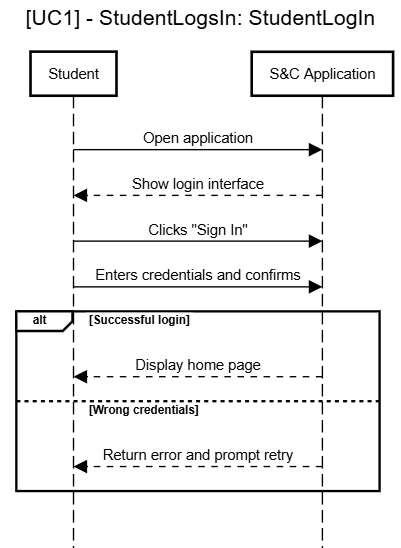
\includegraphics [width=.7\linewidth] {UC1.png}
    \caption{Student Login}
\end{figure}

\begin{figure} [H]
    \centering
    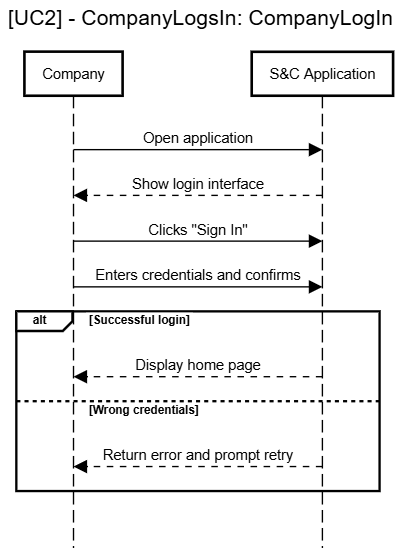
\includegraphics [width=.7\linewidth] {UC2.png}
    \caption{Company Login}
\end{figure}

\begin{figure} [H]
    \centering
    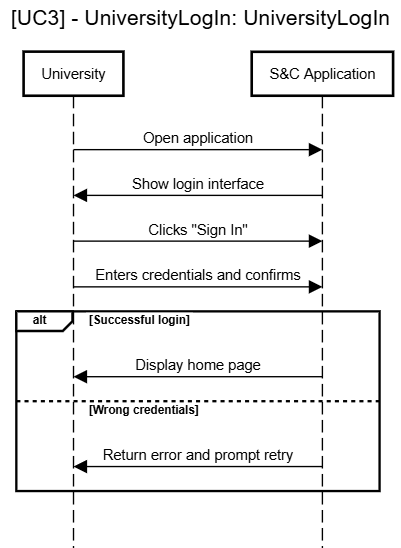
\includegraphics [width=.7\linewidth] {UC3.png}
    \caption{University Login}
\end{figure}

\begin{figure} [H]
    \centering
    
    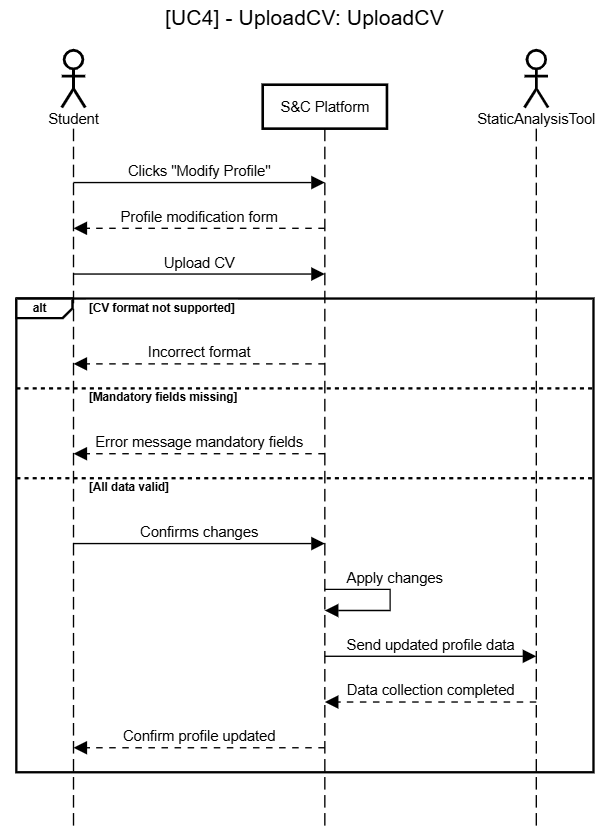
\includegraphics [width=.7\linewidth] {UC4.png}
    \caption{Upload CV}
\end{figure}

\begin{figure} [H]
    \centering
    
    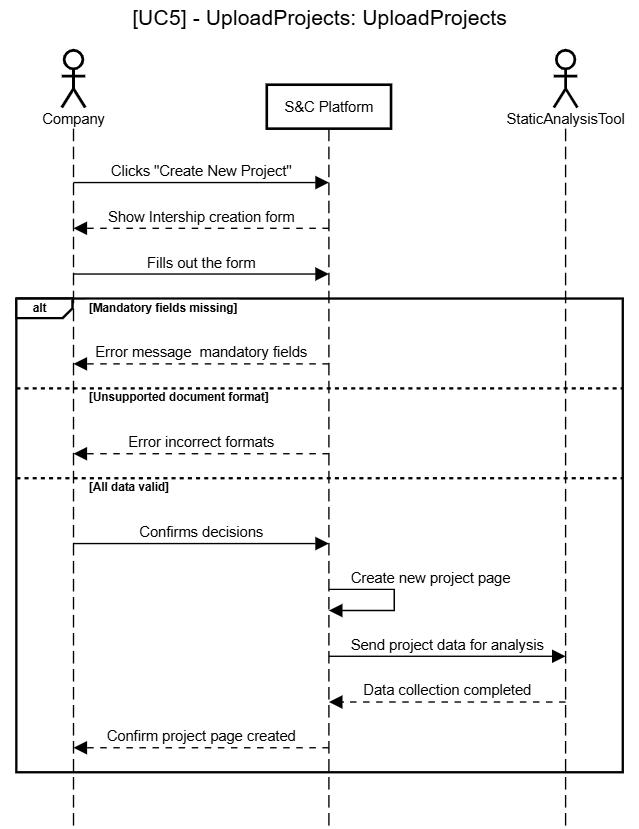
\includegraphics [width=.7\linewidth] {UC5.png}
    \caption{Upload Projects}
\end{figure}

\begin{figure} [H]
    \centering
    
    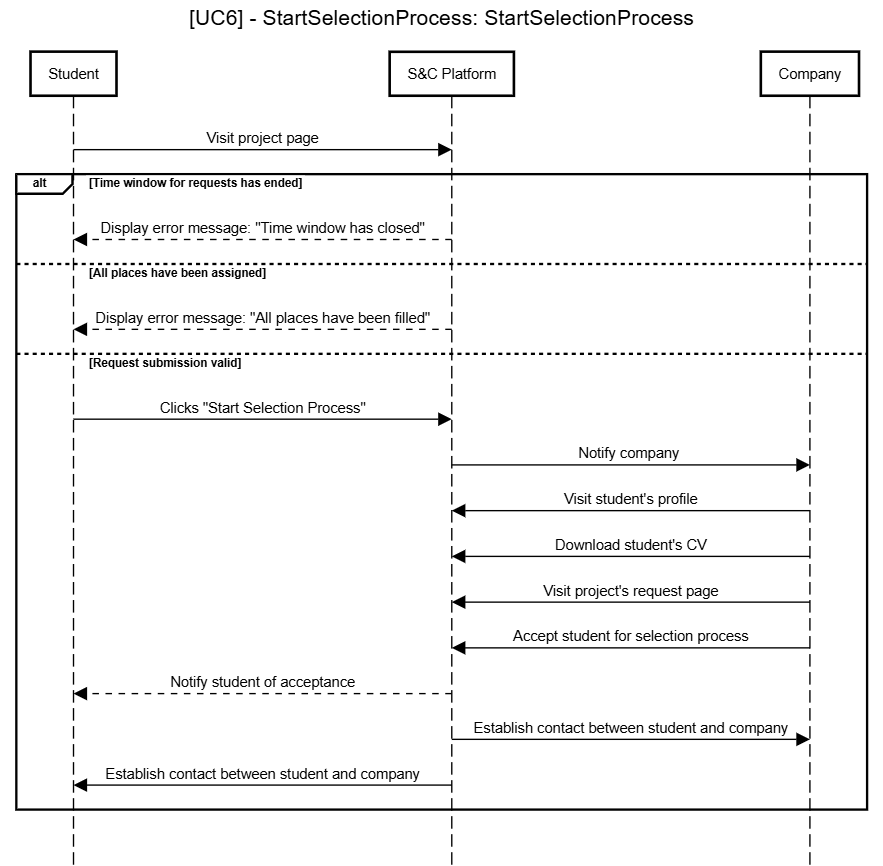
\includegraphics [width=.7\linewidth] {UC6.png}
    \caption{Start Selection Process}
\end{figure}

\begin{figure} [H]
    \centering
    
    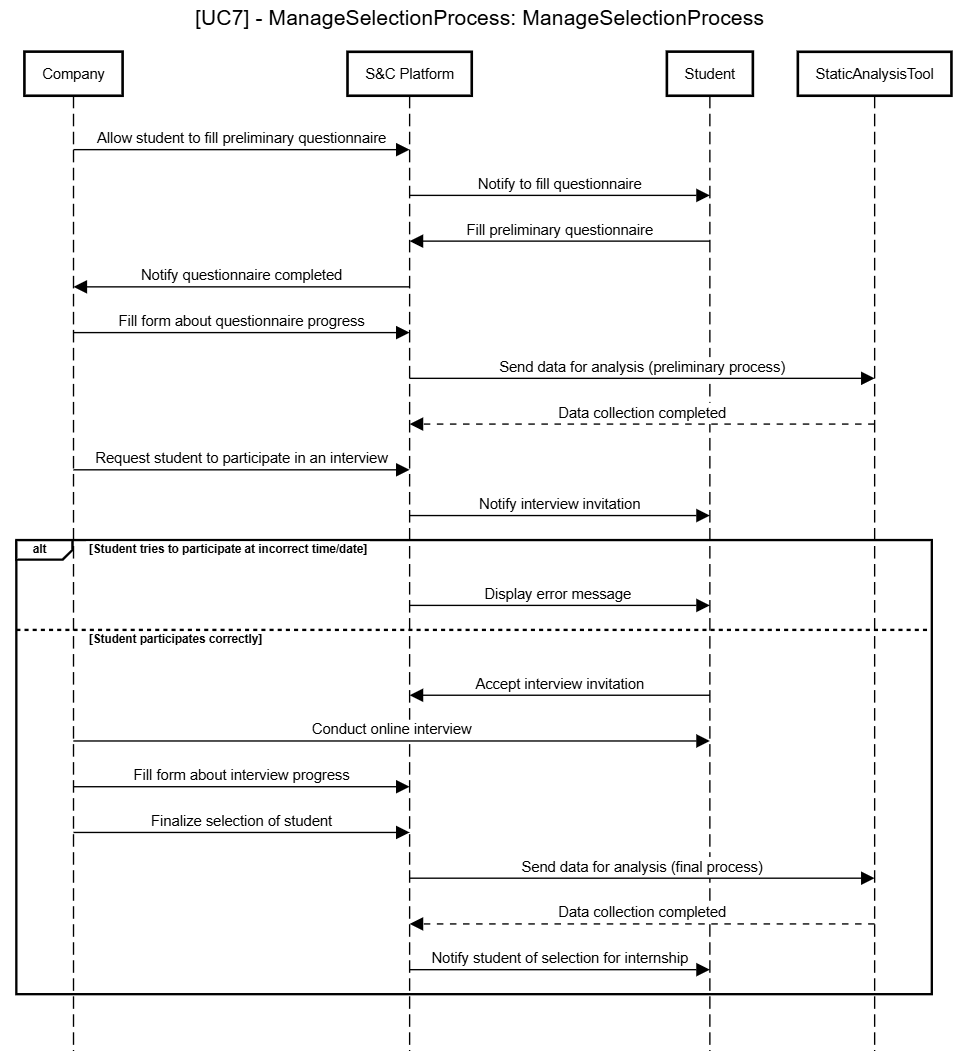
\includegraphics [width=.7\linewidth] {UC7.png}
    \caption{Manage Selection Process}
\end{figure}

\begin{figure} [H]
    \centering
    
    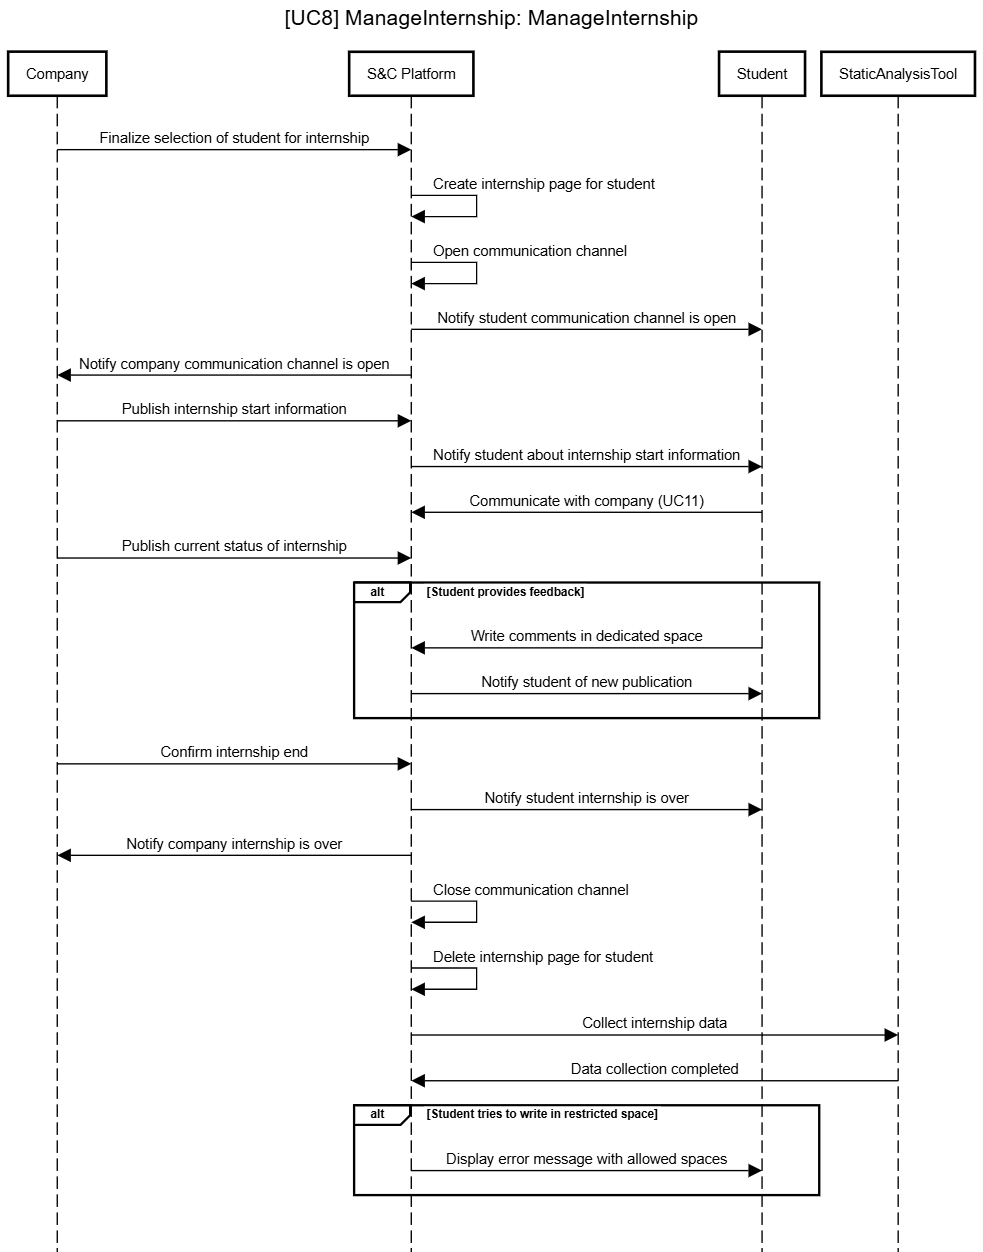
\includegraphics [width=.7\linewidth] {UC8.png}
    \caption{Manage Internship}
\end{figure}

\begin{figure} [H]
    \centering
    
    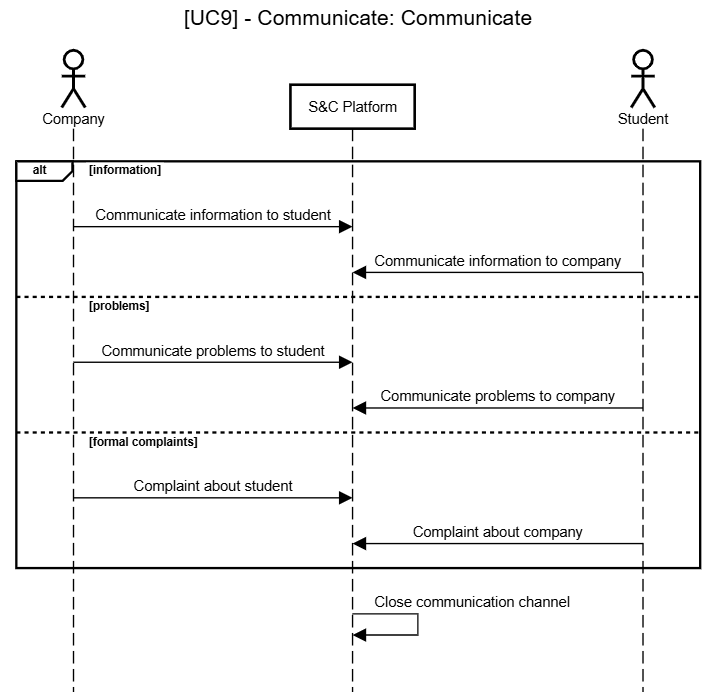
\includegraphics [width=.7\linewidth] {UC9.png}
    \caption{Communicate}
\end{figure}

\begin{figure} [H]
    \centering
    
    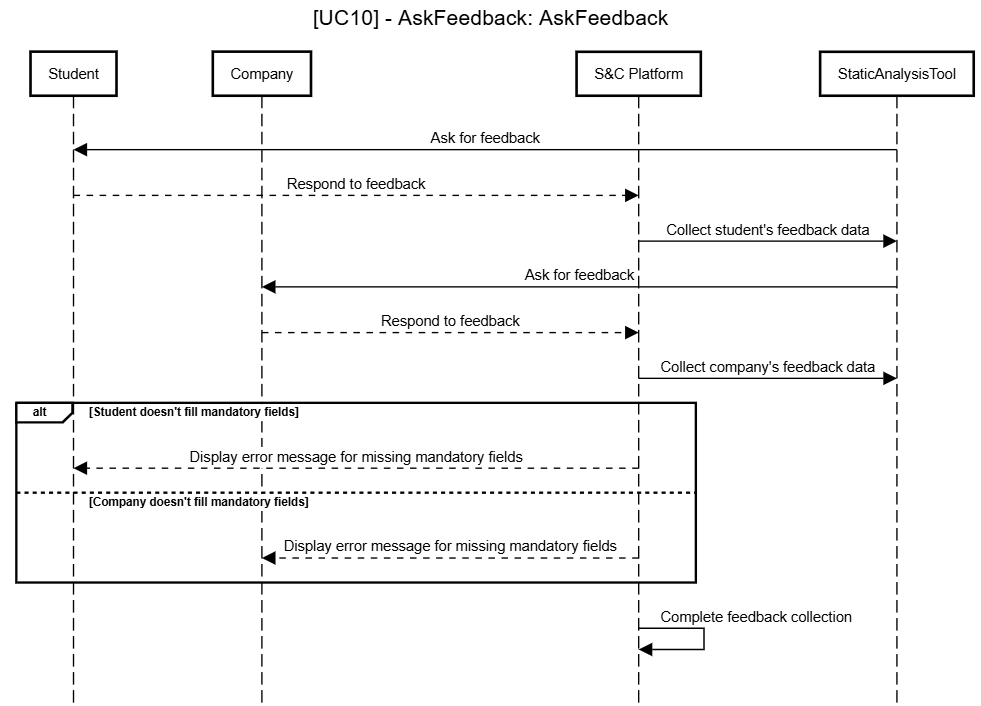
\includegraphics [width=.7\linewidth] {UC10.png}
    \caption{Ask Feedback}
\end{figure}

\begin{figure} [H]
    \centering
    
    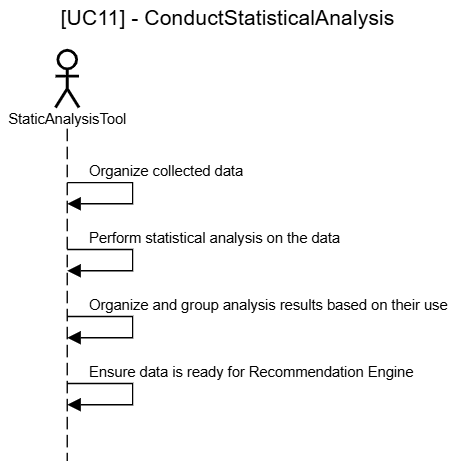
\includegraphics [width=.7\linewidth] {UC11.png}
    \caption{Conduct Statistical Analysis}
\end{figure}

\begin{figure} [H]
    \centering
    
    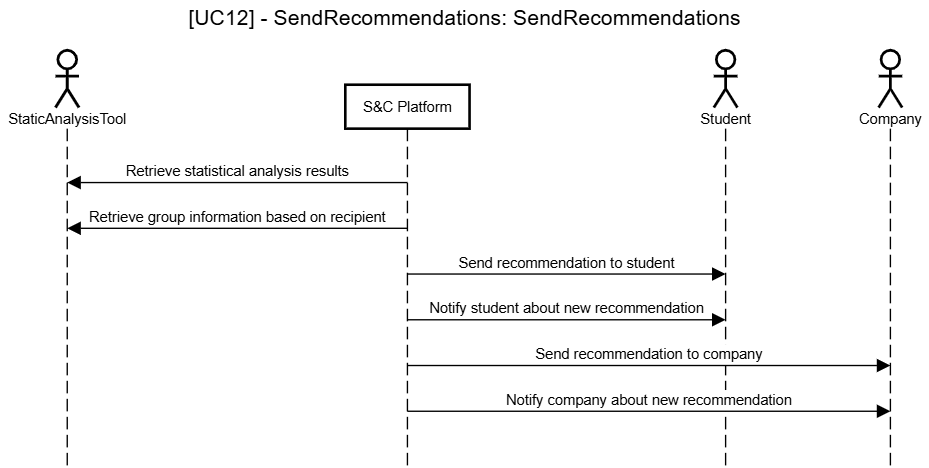
\includegraphics [width=.7\linewidth] {UC12.png}
    \caption{Send Reccommendations}
\end{figure}

\begin{figure} [H]
    \centering
    
    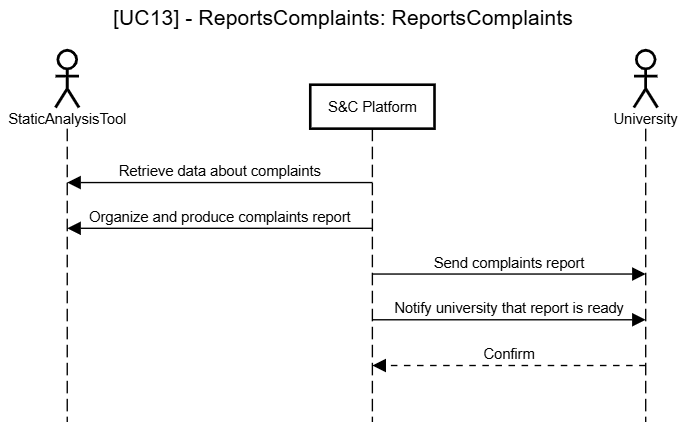
\includegraphics [width=.7\linewidth] {UC13.png}
    \caption{Reports Complaints}
\end{figure}

\begin{figure} [H]
    \centering
    
    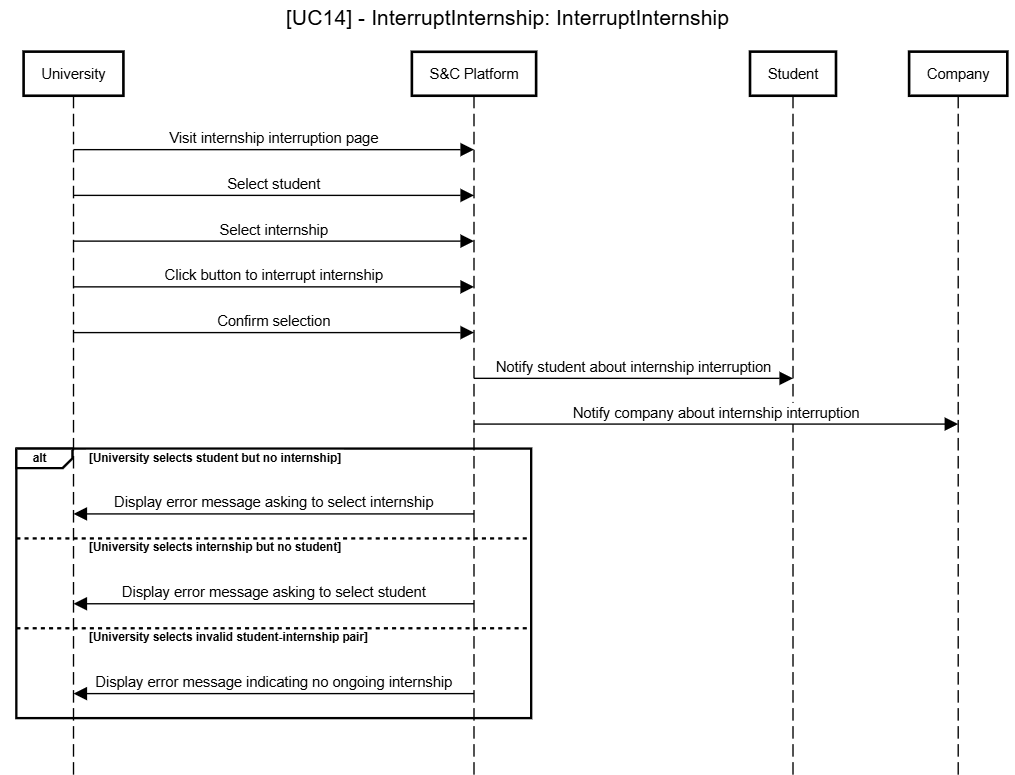
\includegraphics [width=.7\linewidth] {UC14.png}
    \caption{Interrupt Internship}
\end{figure}


\subsection{Activity Diagrams}
\subsection{Requirements Mapping}

\section{Performance Requirements}

\section{Design Constraints}
\subsection{Standard Compliance}
\subsection{Hardware Limitations}
\subsection{Other Constraints}

\section{Software System Attributes}
\subsection{Reliability}
\subsection{Availability}
\subsection{Security}
\subsection{Maintainability}
\subsection{Portability}